\documentclass{article}
\usepackage{tikz}
\begin{document}
\begin{center}
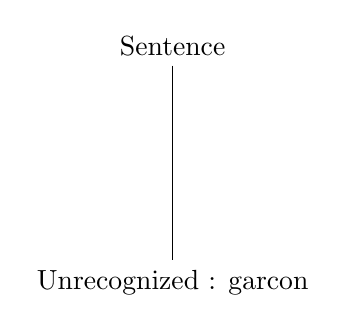
\begin{tikzpicture}
\node{Sentence}[sibling distance = 3cm, level distance = 3cm, align=center]
child {node {Unrecognized : garcon}};
\end{tikzpicture}
\end{center}
\begin{center}
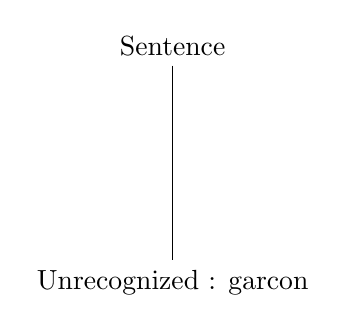
\begin{tikzpicture}
\node{Sentence}[sibling distance = 3cm, level distance = 3cm, align=center]
child {node {Unrecognized : garcon}};
\end{tikzpicture}
\end{center}
\begin{center}
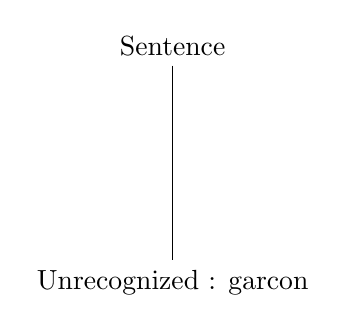
\begin{tikzpicture}
\node{Sentence}[sibling distance = 3cm, level distance = 3cm, align=center]
child {node {Unrecognized : garcon}};
\end{tikzpicture}
\end{center}
\begin{center}
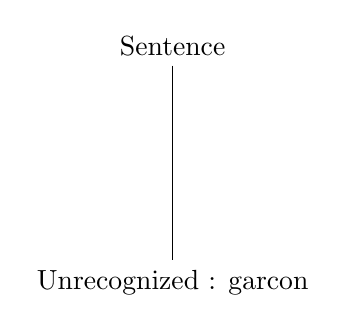
\begin{tikzpicture}
\node{Sentence}[sibling distance = 3cm, level distance = 3cm, align=center]
child {node {Unrecognized : garcon}};
\end{tikzpicture}
\end{center}
\begin{center}
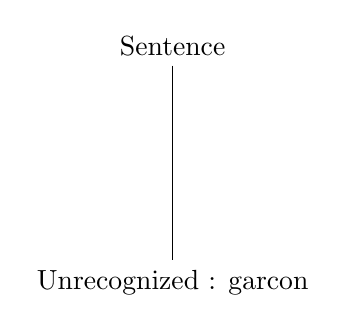
\begin{tikzpicture}
\node{Sentence}[sibling distance = 3cm, level distance = 3cm, align=center]
child {node {Unrecognized : garcon}};
\end{tikzpicture}
\end{center}
\begin{center}
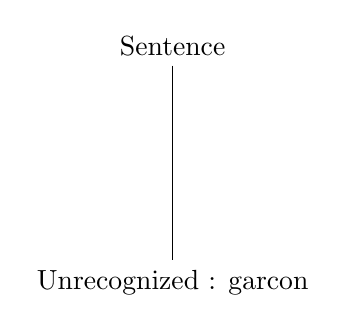
\begin{tikzpicture}
\node{Sentence}[sibling distance = 3cm, level distance = 3cm, align=center]
child {node {Unrecognized : garcon}};
\end{tikzpicture}
\end{center}
\end{document}